\section{Task Decomposition}

Modularization is one approach to reduce the dimension of the state space. In
this section, we will discuss some major approaches of MDP decomposition as
solutions to the curse of dimensionality. We will discuss a hierarchical
approach and a layered approach.

Some complex tasks have explicit phases. Take the taxi domain for example
(Figure~\ref{fig:taxi}). The taxi driver picks up a passenger from a location,
and drives and drops him at a different location. This task requires some shared
low-level skills. Hierarchical RL

\begin{figure}[h]
\centering
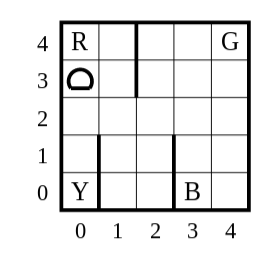
\includegraphics[width=0.3\textwidth]{taxi.png}
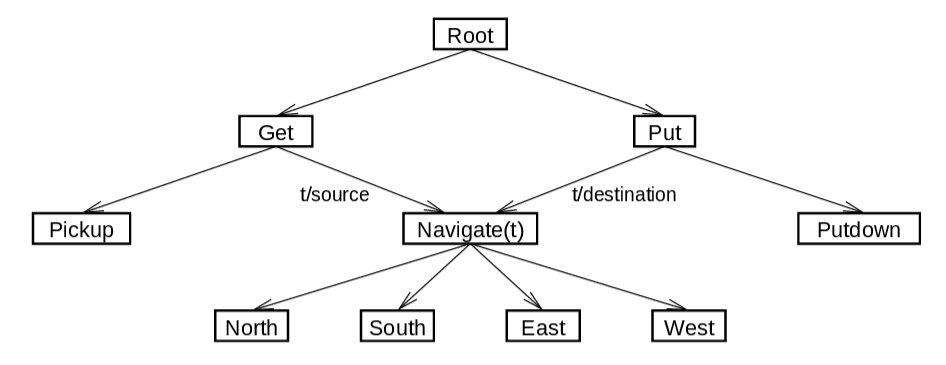
\includegraphics[width=0.6\textwidth]{maxq.png}
\caption{(Left) Taxi domain. (Right) A decomposition of the task.}
\label{fig:taxi}
\vspace{-0.25cm}
\end{figure}

Another popular method, skill switching, also lays in hierarchical RL. 

Hierarchical reinforcement learning is different from modular reinforcement
learning in a way that the former approach doesn't involve concurrent modules
(or sutasks, skills, depending on context).
For example, the Pickup module doesn't run parallel with Navigate module.
Therefore, there is no compromise in policies proposed by different modules.

Layered learning.

Layered learning is similar to modular reinforcement learning, as the modules are
run in parallel. However different modules correspond to different controllers. 

Not fix a model.

\section{Inverse Reinforcement Learning}

We introduced basic concepts of inverse reinforcement learing in the last
chapter. In this section, we discuss some advances in IRL and compare them with
our methods.

assume prior.
